\section{Task Execution and Observation} \label{sec:results_game}
    The game is played twice by the volunteers, once with some initial direction by the observing researcher, and then again without any aid, unless if requested. During the game, the observer’s role is to record the volunteer’s performance in completing the task. Tracking their total game time, their completion time per task, the number of errors they commit, when they have requested help, which tasks the players couldn’t solve correctly, how often the system has caused issues to the players. However, they’re also there to provide support if necessary, and to keep the volunteer sharing about their impressions, as other valuable information may be better accumulated during the process of the play session itself.\\

\subsection{Movement and Time as a Measure } \label{sec:results_game_movementtime}
    One of the elements that the observation was meant to register was the total time taken to complete the game, which would be a function of how fast the players managed to learn and recall the task completion gestures. However, this ended up being moreover, influenced by time taken moving around the virtual environment.\\
    Both times taken to complete tasks and times taken to become accustomed to movement were predicted as important values to take in consideration, however, this latter wasn’t an important metric, as movement had the same approach on both the Cultural and Non-Cultural Groups. It was going to be tracked in the interest of showing important observation, it became clear that doing so the intended way was going to be impossible. Several volunteers never found a moment where they said they got used to the controls to the very end of the experience, and even found trouble the second time. Meanwhile, other users were immediately proficient with it. Nevertheless, all of them still claimed that the movement was the least enjoyable part of the game. The main complication stated being the transition between the left movement and the right movement, as transitioning between the two involved doing too wide of a movement, and the camera wouldn’t pick up on it right away.\\
    But moreover, the most impactful effect of movement over the data was that it made the total game time a noisy metric. Rather being able to take that information and attribute a conclusion to the cultural impact, partial conclusions about technological impact needed to be made as this provides a clear influence. Total times in the first trial were much slower for the Non-Cultural Group Volunteer, but there’s a lot of variance to the values, and for the second trial the values were all much too similar between the two groups, without it being possible to support any conclusion in regard to the change. Individual conclusions may be made, as the fastest times observed in the first trial belong to users reportedly with a high technological interest score (V1, V8, V15), and two proven to be outstandingly fast in the second trial again (V8, V15). Also, there is a user (V9) that was outstandingly slow in the second trial, and who struggled with movement to a much larger extent than everyone in both groups, who coincidentally also reported to have a lower technological interest score than the median. In effect, this user may have struggled with retention of this aspect of the game. However, the lowest times on both trials do not have a definite pattern to the technological interest scores, and even the volunteer who showcased most trouble did not self-report the lowest of all scores. It’s very possible that a correlation exists for higher user confidence with technology and gestural command retention, but, given that technological impact was not the focus of this study and given that the not enough rigor on the was employed to explore the matter and circumvent the potential issue of self-reporting biases, any further analysis was dropped. Reiterating, the thought given to this section is a justification of why movement timing observations were not entirely helpful in drawing meaningful conclusions.\\
    For clarity, table \ref{tab:Table_TotalGameTimes} shows the Total Game Time data of every participant including averages and standard deviation on that data.\\
    
    \begin{table}[ht]
    \begin{tabular}{lllllllll}
    \multicolumn{2}{l}{First Trial}                                   &                                &                                 &                       & \multicolumn{2}{l}{Second Trial}                                 &                                &                                 \\ \cline{2-2} \cline{4-4} \cline{7-7} \cline{9-9} 
    \multicolumn{1}{l|}{Cultural}           & \multicolumn{1}{l|}{Total Time} & \multicolumn{1}{l|}{Non-Cultural}          & \multicolumn{1}{l|}{Total Time} &                       & \multicolumn{1}{l|}{Cultural}          & \multicolumn{1}{l|}{Total Time} & \multicolumn{1}{l|}{Non-Cultural}          & \multicolumn{1}{l|}{Total Time} \\ \cline{1-4} \cline{6-9} 
    \multicolumn{1}{|l|}{V1}        & \multicolumn{1}{l|}{322}        & \multicolumn{1}{l|}{V2}        & \multicolumn{1}{l|}{642}        & \multicolumn{1}{l|}{} & \multicolumn{1}{l|}{V1}        & \multicolumn{1}{l|}{357}        & \multicolumn{1}{l|}{V2}        & \multicolumn{1}{l|}{315}        \\ \cline{1-4} \cline{6-9} 
    \multicolumn{1}{|l|}{V3}        & \multicolumn{1}{l|}{348}        & \multicolumn{1}{l|}{V4}        & \multicolumn{1}{l|}{550}        & \multicolumn{1}{l|}{} & \multicolumn{1}{l|}{V3}        & \multicolumn{1}{l|}{329}        & \multicolumn{1}{l|}{V4}        & \multicolumn{1}{l|}{361}        \\ \cline{1-4} \cline{6-9} 
    \multicolumn{1}{|l|}{V5}        & \multicolumn{1}{l|}{355}        & \multicolumn{1}{l|}{V7}        & \multicolumn{1}{l|}{433}        & \multicolumn{1}{l|}{} & \multicolumn{1}{l|}{V6}        & \multicolumn{1}{l|}{372}        & \multicolumn{1}{l|}{V7}        & \multicolumn{1}{l|}{388}        \\ \cline{1-4} \cline{6-9} 
    \multicolumn{1}{|l|}{V6}        & \multicolumn{1}{l|}{405}        & \multicolumn{1}{l|}{V8}        & \multicolumn{1}{l|}{356}        & \multicolumn{1}{l|}{} & \multicolumn{1}{l|}{V9}        & \multicolumn{1}{l|}{530}        & \multicolumn{1}{l|}{V8}        & \multicolumn{1}{l|}{258}        \\ \cline{1-4} \cline{6-9} 
    \multicolumn{1}{|l|}{V9}        & \multicolumn{1}{l|}{415}        & \multicolumn{1}{l|}{V10}       & \multicolumn{1}{l|}{470}        & \multicolumn{1}{l|}{} & \multicolumn{1}{l|}{V11}       & \multicolumn{1}{l|}{327}        & \multicolumn{1}{l|}{V10}       & \multicolumn{1}{l|}{321}        \\ \cline{1-4} \cline{6-9} 
    \multicolumn{1}{|l|}{V11}       & \multicolumn{1}{l|}{336}        & \multicolumn{1}{l|}{V12}       & \multicolumn{1}{l|}{355}        & \multicolumn{1}{l|}{} & \multicolumn{1}{l|}{V13}       & \multicolumn{1}{l|}{307}        & \multicolumn{1}{l|}{V12}       & \multicolumn{1}{l|}{304}        \\ \cline{1-4} \cline{6-9} 
    \multicolumn{1}{|l|}{V13}       & \multicolumn{1}{l|}{446}        & \multicolumn{1}{l|}{V14}       & \multicolumn{1}{l|}{556}        & \multicolumn{1}{l|}{} & \multicolumn{1}{l|}{V15}       & \multicolumn{1}{l|}{267}        & \multicolumn{1}{l|}{V14}       & \multicolumn{1}{l|}{358}        \\ \cline{1-4} \cline{6-9} 
    \multicolumn{1}{|l|}{V15}       & \multicolumn{1}{l|}{322}        & \multicolumn{1}{l|}{V16}       & \multicolumn{1}{l|}{361}        & \multicolumn{1}{l|}{} & \multicolumn{1}{l|}{V17}       & \multicolumn{1}{l|}{347}        & \multicolumn{1}{l|}{V16}       & \multicolumn{1}{l|}{314}        \\ \cline{1-4} \cline{6-9} 
    \multicolumn{1}{|l|}{V17}       & \multicolumn{1}{l|}{425}        &                                &                                 &                       &                                &                                 &                                &                                 \\ \cline{1-2} \cline{6-9} 
                                    &                                 &                                &                                 & \multicolumn{1}{l|}{} & \multicolumn{1}{l|}{Average}   & \multicolumn{1}{l|}{354.5}      & \multicolumn{1}{l|}{Average}   & \multicolumn{1}{l|}{327.38}     \\ \cline{1-4} \cline{6-9} 
    \multicolumn{1}{|l|}{Average}   & \multicolumn{1}{l|}{374.89}     & \multicolumn{1}{l|}{Average}   & \multicolumn{1}{l|}{465.38}     & \multicolumn{1}{l|}{} & \multicolumn{1}{l|}{Std. Dev.} & \multicolumn{1}{l|}{77.91}      & \multicolumn{1}{l|}{Std. Dev.} & \multicolumn{1}{l|}{40.49}      \\ \cline{1-4} \cline{6-9} 
    \multicolumn{1}{|l|}{Std. Dev.} & \multicolumn{1}{l|}{47.84}      & \multicolumn{1}{l|}{Std. Dev.} & \multicolumn{1}{l|}{108.68}     &                       &                                &                                 &                                &                                 \\ \cline{1-4}
    \end{tabular}
    \caption{\label{tab:Table_TotalGameTimes}Total elapsed time between game start and completion of both Cultural and Non-Cultural Groups for both First and Follow-Up Trial's observations}
    \end{table}
    
\subsection{Volunteer Number 8} \label{sec:results_game_volunteernumber8}
    Volunteer number 8 stands out as an unexpected anomaly to the data. To better highlight why this is the case, the following table \ref{tab:Table_Volunteer 8} is collated to the document. It should be noted that, for the purposes of better showcasing the difference between this one and the other volunteers in the Non-Cultural Group, data from the O2 and T2 tasks was not left out.\\
    
    \begin{table}[ht]
    \begin{tabular}{|l|l|l|l|}
    \hline
    & Total User Errors & Total Forgotten Gestures & Total Help Requests \\ \hline
    V2  & 5                 & 4                        & 0                   \\ \hline
    V4  & 8                 & 4                        & 1                   \\ \hline
    V7  & 6                 & 4                        & 0                   \\ \hline
    \rowcolor[HTML]{e2ffe1} 
    V8  & 0                 & 0                        & 0                   \\ \hline
    V10 & 4                 & 4                        & 0                   \\ \hline
    V12 & 7                 & 7                        & 1                   \\ \hline
    V14 & 8                 & 3                        & 2                   \\ \hline
    V16 & 6                 & 3                        & 1                   \\ \hline
    \end{tabular}
    \caption{\label{tab:Table_Volunteer 8}Count of focused performance failures commited by Non-Cultural Group members during the Second Trial}
    \end{table}
    
    Despite being in a group that consistently showcases struggles with the game, Volunteer number 8 has performed no observable mistakes. Additionally, they were also the fastest of all participants in completing the tasks and were one of the fastest users in getting used to the movement options. And in the first trial, they may have committed user errors, but all of them were related to aid requests and ensuring they were not about to perform an error ahead of time. Similarly, all delays in completing any of the Tasks by the user were due to them taking a moment to think and recall on their own, and they have removed their hand from within the Leap Motion’s tracking radius to prevent any accidental reading. In other words, they learned the system’s functions and restrictions instantly.\\ 
    Nonetheless, they claimed to have never experimented with systems entirely controlled by means of hand gestures, and to have a low amount of experience with other similar ones, such as Virtual Reality environments with hand tracking controllers. They did however, state that they had a larger degree of experience with consoles with wide arm gestures such as the Nintendo’s Wiimote, but claimed to have never tried the more similar tracking approach used by the Sony Move. Thus, the major characteristic the user had going for them, was their earlier self-reported high interest in the field of Human Interaction, and their efforts towards it given their study of technology at the same university the trials were performed in.\\
    In terms of determining if the user is a statistical outlier, the data changes slightly depending based on whether or not the full sample of data from both trials is used or not. Assuming a Normal Distribution of users, the probability of the user’s Standard Score being observed is below 3.44\% (-2.124) with data from both trials and below 1.70\% (-1.828) taking data from only the second trial. Additionally, the level of technological interest showcased is above 2,794\% (1.886). There’s enough of a suspicion the user lands two standard deviations above the median in performance, however, choosing a correct cut-off is a well-known matter known to produce false positives in a test group with low amount number of test items or low population \cite{hambleton1978use} \cite{ingraham1996empirical}. With two oddities among score on a two-tailed cut-off, there’s still least a 5\% chance that the user was incorrectly leveraged as an outlier, and the rigor self-employed in determining further measures beyond performance errors is of question, as well as the potential misgivings of the sample size or methodology. As such, despite the tabled data crossing the 0.05 alpha level on a two tailed cut-off (+/- 1.96) for the second trial on its own, there’s a fear that eliminating the user may be a mistake on the part of the analysis.\\

\subsection{Performances, Memory and User Errors} \label{sec:results_game_performance}
    
    User performance was registered during the game, this was the focal point of the observation protocol. Odd behaviours, mistakes, failure at remembering the correct gesture and help requests were the primary measures employed, targeted primarily at moments during which Tasks were being completed. Table \ref{tab:Table_Performance} provides an overview of a summary of the data collected for both Cultural and Non-Cultural groups during both of the trials, with the dimensions: Average Task Time, Total Number of User Errors, Total Number of Failures (Didn’t use the correct gesture), Total Number of Help Requests. The choice towards using totals rather than converted scores here is found apt due to both groups having the same size, 8 participants, and thus any pre-processing of the data would just lead to the same results. It ought to be highlighted that additional time information was already noted on \ref{tab:Table_TotalGameTimes}.\\ 
    
    \begin{table}[ht]
    \begin{tabular}{lllllllllllll}
    \cline{2-13}
    \multicolumn{1}{l|}{}     & \multicolumn{4}{l|}{O1}                                                                                         & \multicolumn{4}{l|}{T1}                                                                                         & \multicolumn{4}{l|}{O3}                                                                                        \\ \cline{2-13} 
    \multicolumn{1}{l|}{}     & \multicolumn{1}{l|}{Time}  & \multicolumn{1}{l|}{Error} & \multicolumn{1}{l|}{Fail} & \multicolumn{1}{l|}{Help} & \multicolumn{1}{l|}{Time}  & \multicolumn{1}{l|}{Error} & \multicolumn{1}{l|}{Fail} & \multicolumn{1}{l|}{Help} & \multicolumn{1}{l|}{Time} & \multicolumn{1}{l|}{Error} & \multicolumn{1}{l|}{Fail} & \multicolumn{1}{l|}{Help} \\ \hline
    \multicolumn{1}{|l|}{C1}  & \multicolumn{1}{l|}{8.63}  & \multicolumn{1}{l|}{2}     & \multicolumn{1}{l|}{0}    & \multicolumn{1}{l|}{1}    & \multicolumn{1}{l|}{8.56}  & \multicolumn{1}{l|}{0}     & \multicolumn{1}{l|}{0}    & \multicolumn{1}{l|}{2}    & \multicolumn{1}{l|}{6.22} & \multicolumn{1}{l|}{0}     & \multicolumn{1}{l|}{0}    & \multicolumn{1}{l|}{0}    \\ \hline
    \multicolumn{1}{|l|}{C2}  & \multicolumn{1}{l|}{7.25}  & \multicolumn{1}{l|}{0}     & \multicolumn{1}{l|}{0}    & \multicolumn{1}{l|}{0}    & \multicolumn{1}{l|}{10.88} & \multicolumn{1}{l|}{2}     & \multicolumn{1}{l|}{0}    & \multicolumn{1}{l|}{0}    & \multicolumn{1}{l|}{6.57} & \multicolumn{1}{l|}{2}     & \multicolumn{1}{l|}{0}    & \multicolumn{1}{l|}{0}    \\ \hline
    \multicolumn{1}{|l|}{NC1} & \multicolumn{1}{l|}{10.17} & \multicolumn{1}{l|}{7}     & \multicolumn{1}{l|}{3}    & \multicolumn{1}{l|}{2}    & \multicolumn{1}{l|}{6.75}  & \multicolumn{1}{l|}{1}     & \multicolumn{1}{l|}{1}    & \multicolumn{1}{l|}{1}    & \multicolumn{1}{l|}{5.20} & \multicolumn{1}{l|}{3}     & \multicolumn{1}{l|}{3}    & \multicolumn{1}{l|}{1}    \\ \hline
    \multicolumn{1}{|l|}{NC2} & \multicolumn{1}{l|}{7.50}  & \multicolumn{1}{l|}{6}     & \multicolumn{1}{l|}{3}    & \multicolumn{1}{l|}{0}    & \multicolumn{1}{l|}{8.25}  & \multicolumn{1}{l|}{5}     & \multicolumn{1}{l|}{2}    & \multicolumn{1}{l|}{0}    & \multicolumn{1}{l|}{8.50} & \multicolumn{1}{l|}{8}     & \multicolumn{1}{l|}{6}    & \multicolumn{1}{l|}{2}    \\ \hline
                              &                            &                            &                           &                           &                            &                            &                           &                           &                           &                            &                           &                           \\ \cline{2-13} 
    \multicolumn{1}{l|}{}     & \multicolumn{4}{l|}{T3.1}                                                                                       & \multicolumn{4}{l|}{T3.2}                                                                                       & \multicolumn{4}{l|}{O4}                                                                                        \\ \cline{2-13} 
    \multicolumn{1}{l|}{}     & \multicolumn{1}{l|}{Time}  & \multicolumn{1}{l|}{Error} & \multicolumn{1}{l|}{Fail} & \multicolumn{1}{l|}{Help} & \multicolumn{1}{l|}{Time}  & \multicolumn{1}{l|}{Error} & \multicolumn{1}{l|}{Fail} & \multicolumn{1}{l|}{Help} & \multicolumn{1}{l|}{Time} & \multicolumn{1}{l|}{Error} & \multicolumn{1}{l|}{Fail} & \multicolumn{1}{l|}{Help} \\ \hline
    \multicolumn{1}{|l|}{C1}  & \multicolumn{1}{l|}{6.33}  & \multicolumn{1}{l|}{0}     & \multicolumn{1}{l|}{0}    & \multicolumn{1}{l|}{0}    & \multicolumn{1}{l|}{6.89}  & \multicolumn{1}{l|}{0}     & \multicolumn{1}{l|}{0}    & \multicolumn{1}{l|}{0}    & \multicolumn{1}{l|}{6.33} & \multicolumn{1}{l|}{0}     & \multicolumn{1}{l|}{0}    & \multicolumn{1}{l|}{0}    \\ \hline
    \multicolumn{1}{|l|}{C2}  & \multicolumn{1}{l|}{6.25}  & \multicolumn{1}{l|}{0}     & \multicolumn{1}{l|}{0}    & \multicolumn{1}{l|}{0}    & \multicolumn{1}{l|}{8.88}  & \multicolumn{1}{l|}{0}     & \multicolumn{1}{l|}{0}    & \multicolumn{1}{l|}{0}    & \multicolumn{1}{l|}{6.00} & \multicolumn{1}{l|}{0}     & \multicolumn{1}{l|}{0}    & \multicolumn{1}{l|}{0}    \\ \hline
    \multicolumn{1}{|l|}{NC1} & \multicolumn{1}{l|}{7.50}  & \multicolumn{1}{l|}{5}     & \multicolumn{1}{l|}{2}    & \multicolumn{1}{l|}{2}    & \multicolumn{1}{l|}{11.13} & \multicolumn{1}{l|}{6}     & \multicolumn{1}{l|}{1}    & \multicolumn{1}{l|}{3}    & \multicolumn{1}{l|}{7.00} & \multicolumn{1}{l|}{2}     & \multicolumn{1}{l|}{1}    & \multicolumn{1}{l|}{1}    \\ \hline
    \multicolumn{1}{|l|}{NC2} & \multicolumn{1}{l|}{7.38}  & \multicolumn{1}{l|}{7}     & \multicolumn{1}{l|}{5}    & \multicolumn{1}{l|}{0}    & \multicolumn{1}{l|}{10.25} & \multicolumn{1}{l|}{5}     & \multicolumn{1}{l|}{3}    & \multicolumn{1}{l|}{0}    & \multicolumn{1}{l|}{6.17} & \multicolumn{1}{l|}{5}     & \multicolumn{1}{l|}{5}    & \multicolumn{1}{l|}{0}    \\ \hline
                              &                            &                            &                           &                           &                            &                            &                           &                           &                           &                            &                           &                           \\ \cline{2-5}
    \multicolumn{1}{l|}{}     & \multicolumn{4}{l|}{T4}                                                                                         &                            &                            &                           &                           &                           &                            &                           &                           \\ \cline{2-5}
    \multicolumn{1}{l|}{}     & \multicolumn{1}{l|}{Time}  & \multicolumn{1}{l|}{Error} & \multicolumn{1}{l|}{Fail} & \multicolumn{1}{l|}{Help} &                            &                            &                           &                           &                           &                            &                           &                           \\ \cline{1-5}
    \multicolumn{1}{|l|}{C1}  & \multicolumn{1}{l|}{7.33}  & \multicolumn{1}{l|}{0}     & \multicolumn{1}{l|}{0}    & \multicolumn{1}{l|}{2}    &                            &                            &                           &                           &                           &                            &                           &                           \\ \cline{1-5}
    \multicolumn{1}{|l|}{C2}  & \multicolumn{1}{l|}{11.75} & \multicolumn{1}{l|}{0}     & \multicolumn{1}{l|}{0}    & \multicolumn{1}{l|}{0}    &                            &                            &                           &                           &                           &                            &                           &                           \\ \cline{1-5}
    \multicolumn{1}{|l|}{NC1} & \multicolumn{1}{l|}{8.00}  & \multicolumn{1}{l|}{2}     & \multicolumn{1}{l|}{1}    & \multicolumn{1}{l|}{2}    &                            &                            &                           &                           &                           &                            &                           &                           \\ \cline{1-5}
    \multicolumn{1}{|l|}{NC2} & \multicolumn{1}{l|}{9.25}  & \multicolumn{1}{l|}{1}     & \multicolumn{1}{l|}{1}    & \multicolumn{1}{l|}{0}    &                            &                            &                           &                           &                           &                            &                           &                           \\ \cline{1-5}
    \end{tabular}
    \caption{\label{tab:Table_Performance}User Performance Data during the First and Second Trials.}
    \end{table}
    Of the data displayed, time ended up being the least insightful. It was already discussed prior that total game time did not yield many discernible results due to the influence movement had on the players, without this being one of the differentiated aspects between players. However, discounting all time spent on moving the character, still this doesn’t prove to be a much conclusive metric. By further organizing data and preparing a time comparison table between the Cultural and Non-Cultural Group \ref{fig:FigureTimeComparisonTable}, while it may appear that the Non-Cultural Group has more trouble in quickly solving each of the tasks, this is neither a consistent observation, nor was it possible to prove with 95\% confidence that such was the case. Additionally, it’s not possible to use the data as supporting evidence that the more user error performed by the groups for a task, the slower the group was. Using regressions analysis, the value of R-square is a minute 0.5688, which is far from enough to call a good fit between the two.\\
    \begin{figure}[t]
        \centering
        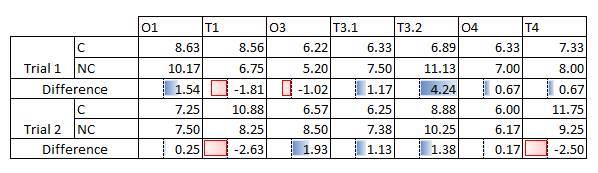
\includegraphics[width=0.8\paperwidth]{figures/TimeComparisonTable.png}
        \caption{\label{fig:FigureTimeComparisonTable}Tast Execution time comparison Table between Cultural and Non-Cultural Groups}
    \end{figure}
    Naturally, that does seem to point out that fitting Cultural Emblems are a beneficial method of approaching a gestural control scheme, as it seems to lower the negative impact seen both aspects for the Non-Cultural Group. However, there needs to be a tell that makes that clear within the data. To that end, the mistakes committed by this Non-Cultural Group need to be looked at. Were they making a mistake because of the difficulty of the Gestures themselves? Were they confusing the correct gesture from another Task with the one they were trying to Solve? As such, all Non-Cultural Group’s erroneous gestures were registered and looked, and with that, the break-down table \ref{tab:Table_ErrorBreakdown} was made, manifesting the most conspicuous of type of error.\\
    
    \begin{table}[t]
    \begin{tabular}{llllllll}
    \cline{2-8}
    \multicolumn{1}{l|}{}                                   & \multicolumn{1}{l|}{O1} & \multicolumn{1}{l|}{T1} & \multicolumn{1}{l|}{O3} & \multicolumn{1}{l|}{T3.1} & \multicolumn{1}{l|}{T3.2} & \multicolumn{1}{l|}{O4} & \multicolumn{1}{l|}{T4} \\ \hline
    \multicolumn{1}{|l|}{Total Mistakes}                    & \multicolumn{1}{l|}{6}  & \multicolumn{1}{l|}{5}  & \multicolumn{1}{l|}{8}  & \multicolumn{1}{l|}{7}    & \multicolumn{1}{l|}{5}    & \multicolumn{1}{l|}{5}  & \multicolumn{1}{l|}{1}  \\ \hline
    \multicolumn{1}{|l|}{Gestural Mistakes}                 & \multicolumn{1}{l|}{6}  & \multicolumn{1}{l|}{4}  & \multicolumn{1}{l|}{3}  & \multicolumn{1}{l|}{5}    & \multicolumn{1}{l|}{4}    & \multicolumn{1}{l|}{5}  & \multicolumn{1}{l|}{1}  \\ \hline
    \multicolumn{1}{|l|}{Emblematic Substitutions}          & \multicolumn{1}{l|}{6}  & \multicolumn{1}{l|}{3}  & \multicolumn{1}{l|}{2}  & \multicolumn{1}{l|}{5}    & \multicolumn{1}{l|}{4}    & \multicolumn{1}{l|}{5}  & \multicolumn{1}{l|}{1}  \\ \hline
    \multicolumn{1}{|l|}{External Emblematic Substitutions} & \multicolumn{1}{l|}{2}  & \multicolumn{1}{l|}{1}  & \multicolumn{1}{l|}{2}  & \multicolumn{1}{l|}{0*}   & \multicolumn{1}{l|}{4}    & \multicolumn{1}{l|}{3}  & \multicolumn{1}{l|}{1}  \\ \hline
    \multicolumn{8}{l}{* All 5 performed the same gesture: Wave; And didn't realize it was wrong.}
    \end{tabular}
    \caption{\label{tab:Table_ErrorBreakdown}Breakdown of Error Types made by the Non-CulturalGroup in the second trial.}
    \end{table}
    Of all the mistakes committed, roughly 75\% were Gestural mistakes. These are when the user attempts to perform a gesture that is wrong for the Task and doesn't stop their attempt until after completing the gesture. The remaining 25\% are other types of mistakes which also include errors related to gestures, but that did not involve a full attempt with that given wrong gesture. Now, of these 28 Gestural Mistakes, all except 2 were Emblematic Substitutions. Here, Emblematic Substitutions are mistakes where the volunteer performed an emblem belonging to their culture instead of the requested command, and as would be expected, their choice of Emblems for the task was for the most part, chosen from among gestures the volunteers had performed during their initial Cultural Survey in the pre-test. What this seems to imply is, despite being told clearly not to use those emblems as they would be considered wrong, the participants' memory still made them recall their emblematic gestures over the gesture they actually performed the first time they performed the game. Which is evidence that Emblems are the more natural way performing those tasks. For clarity, the 2 non-emblematic gestures involved Pantomimes, one with the user attempting to say "here" while pointing out proximity to themselves with their hand, and another outright performing Mimicry, grabbing and dragging an invisible object.\\
    The final row refers to External Emblematic Substitutions. Here, the word External refers to the Game's gestural command set, and thus, this breaks downs how many of the Emblematic Substitutions brought gestures that weren't present on the game at all. What's important about this difference, is to show how many of the above were split between merely forgetting the gesture and attempting to solve it in the way felt right, or how many actually recalled performing a certain gesture, and were trying to fit it within a context that made sense. One such example of the latter was the Task O1, as all 4 of the non-external substitutions involved the volunteers performing Task O2's gesture, thus, it's very likely that all 4 of these volunteers were trying to recontextualize a gesture they knew rather than successfully recalling the correct gesture taught. Meanwhile, the other two participants that did use an External gesture, performed what would have been the Cultural Groups' command. More on this will be brought up on section \ref{sec:results_surveys_confidence}.\\ 
    This row, however, is a bit open to interpretation, namely in regard to Task T3.1. Also noted in the table, all 5 users performed the exact same mistake of doing a Wave motion to solve this task, which is the method by which two other tasks are solved in the Non-Cultural Group. What's noteworthy about Task T3.1 is it involves calling the attention of a blue humanoid helper that is fully animated in reaction to the participants. And one of the actions this animated helper performs to the player once their attention was caught, is Waving their hand in front of its face. There's a strong reason to believe that the users were actually recalling the response of the helper, rather than misremembering the context in which a waving gesture fits within the game.\\
    Ultimately, nearly every substitution ended up resembling the users Cultural Surveys or even the Cultural Group's gesture set. There are strong reasons to believe that well-fitting Emblematic Gestures had an impact in both the short-term learning attainment rate of the game's gesture set, but also of the long term memorization, against lesser-fitting emblematic or options.\\